\documentclass{beamer}


\usepackage{amsmath}
\usepackage[style=alphabetic,url=true]{biblatex}
\usepackage{environ}
\usepackage{geometry}
\usepackage{graphicx}
\usepackage{tikz}
\usepackage[T2A]{fontenc}
\usepackage[utf8]{inputenc}
\usepackage[cache=false]{minted}
\usepackage{amsmath}
\usepackage{amsfonts}
\usepackage{amssymb}
\usepackage{calrsfs}


% \usetheme{Bergen}

\usecolortheme{beaver}

\setbeamertemplate{itemize item}[circle]
\setbeamertemplate{itemize subitem}{--}
\addtobeamertemplate{navigation symbols}{}{
  \usebeamerfont{footline}%
  \usebeamercolor[fg]{footline}%
  \hspace{1em}%
  \insertframenumber/\inserttotalframenumber
}
\graphicspath{ {./graphics/} }
\setminted[Python]{
  fontsize=\tiny
}
\BeforeBeginEnvironment{minted}{\medskip}
\AfterEndEnvironment{minted}{\medskip}
\usetikzlibrary{matrix}
\tikzset{
  stack/.style={
    matrix of nodes,
    nodes={
      fill=lightgray,draw,text=black,font=\sffamily\bfseries,
      text height=11pt,text depth=3pt,baseline=center, minimum width=1cm
    },
    column sep=-\pgflinewidth/2
  }
}

\title{
  Bitcoin and Cryptocurrency Technologies \\
  Lecture 5: Bitcoin Transactions
}

\author{Yuri Zhykin}
\date{Mar 22, 2021}

\begin{document}

\frame{\titlepage}

\begin{frame}
  \frametitle{Transaction Structure}
  \begin{itemize}
  \item \textbf{Tx}
    \begin{itemize}
    \item \textbf{version}
    \item \textbf{inputs} (list of \textbf{TxInput}s)
    \item \textbf{outputs} (list of \textbf{TxOutput}s)
    \item \textbf{witnesses} (list of \textbf{Witness}es)
    \item \textbf{locktime}
    \end{itemize}
  \item \textbf{TxInput}
    \begin{itemize}
    \item \textbf{previous-tx-id}
    \item \textbf{previous-tx-index}
    \item \textbf{unlock-script}
    \end{itemize}
  \item \textbf{TxOutput}
    \begin{itemize}
    \item \textbf{amount}
    \item \textbf{lock-script}
    \end{itemize}
  \end{itemize}
\end{frame}

\begin{frame}[fragile]
  \frametitle{Transfer of Ownership}
  \begin{itemize}
  \item Unspent transaction outputs (\textbf{UTXOs}) are records of bitcoin
    ownership - bitcoin is locked to owners via lock-scripts.
  \item Bitcoin transactions transfer bitcoin by \textit{destroying} subsets of
    all unspent \textit{outputs} (by providing \textit{inputs} that unlock the
    output scripts) and creating new unspent \textit{outputs}.
  \end{itemize}
  \begin{center}
    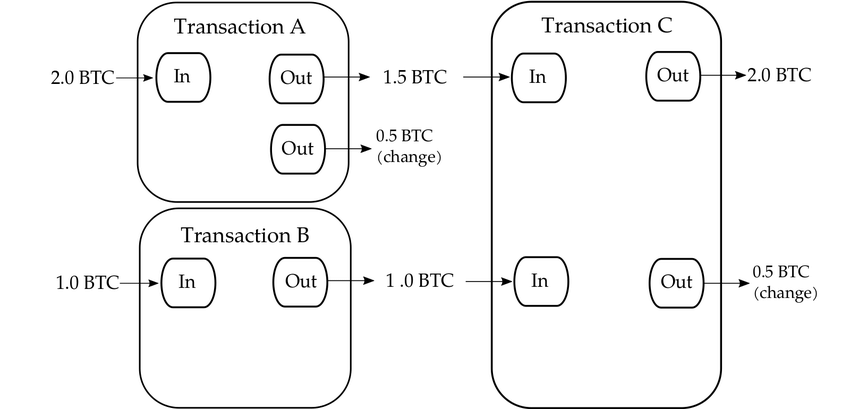
\includegraphics[width=0.8\textwidth]{transactions}
  \end{center}
\end{frame}

\begin{frame}[fragile]
  \frametitle{Bitcoin Script}
  \begin{itemize}
  \item \textbf{Bitcoin Script} or simply \textbf{Script} is a
    \textbf{stack-based} \textbf{Forth-like} \textbf{Turing-incomplete} language
    for expressing locking/unlocking logic in Bitcoin transactions.
  \item Script provides flexibility in defining the conditions for spending each
    particular ``chunk'' of bitcoin.
  \item Because of \textit{Proof-of-Work}, Bitcoin is a first decentralized
    money system, but because of \textit{Script} it is also the first
    \textbf{programmable} money system.
  \end{itemize}
\end{frame}

\begin{frame}[fragile]
  \frametitle{Stack-based Programming}
  \begin{itemize}
  \item \textbf{Stack-based programming} is a programming paradigm which relies
    on a \textbf{stack machine model} for passing parameters.
  \item Example:
    \begin{enumerate}
    \item
      \begin{tabular}{rl}
        Code &\mintinline[bgcolor=lightgray]{Lisp}{3 5 add 3 mul;} \\
        Data &\mintinline[bgcolor=lightgray]{Lisp}{;} \\
      \end{tabular}
    \item
      \begin{tabular}{rl}
        Code &\mintinline[bgcolor=lightgray]{Lisp}{5 add 3 mul;} \\
        Data &\mintinline[bgcolor=lightgray]{Lisp}{3;} \\
      \end{tabular}
    \item
      \begin{tabular}{rl}
        Code &\mintinline[bgcolor=lightgray]{Lisp}{add 3 mul;} \\
        Data &\mintinline[bgcolor=lightgray]{Lisp}{5 3;} \\
      \end{tabular}
    \item
      \begin{tabular}{rl}
        Code &\mintinline[bgcolor=lightgray]{Lisp}{3 mul;} \\
        Data &\mintinline[bgcolor=lightgray]{Lisp}{8;} \\
      \end{tabular}
    \item
      \begin{tabular}{rl}
        Code &\mintinline[bgcolor=lightgray]{Lisp}{mul;} \\
        Data &\mintinline[bgcolor=lightgray]{Lisp}{3 8;} \\
      \end{tabular}
    \item
      \begin{tabular}{rl}
        Code &\mintinline[bgcolor=lightgray]{Lisp}{;} \\
        Data &\mintinline[bgcolor=lightgray]{Lisp}{24;} \\
      \end{tabular}
    \end{enumerate}
  \end{itemize}
\end{frame}

\begin{frame}[fragile]
  \frametitle{Turing-incompleteness}
  \begin{itemize}
  \item \textit{Script} is \textit{intentionally} Turing-incomplete.
  \item On of the core component of modern programming languages is missing:
    \textbf{loop}.
  \item Scripts in transactions are executed by every validating node on the
    network, so loops could be used as means of DoS-attacking the network.
  \item Loops introduce complexity that is hard to analyse statically (i.e. by
    ``looking'' at the code without executing it).
  \item Ethereum network uses a Turing-complete language \textbf{Solidity},
    which is arguably the reason behind some of the worst security incidents in
    the history of Ethereum.
  \end{itemize}
\end{frame}

\begin{frame}[fragile]
  \frametitle{Bitcoin Script Operations 1/3}
  \begin{itemize}
  \item Script execution is the main part of transaction validation.
  \item \textit{Script interpreter} consists of a stack of commands and a stack
    of data.
  \item For each input in a transaction, it's unlock-script is executed first,
    then the resulting stack is used to execute the lock-script of the
    corresponding output:
    \begin{itemize}
    \item initialize an empty stack $S_0 = S_{empty}$
    \item execute the TxInput's unlock-script on stack $S_0$:
      $$S_1 = Execute(UnlockScript, S_0)$$
    \item execute corresponding TxOutput's lock-script on stack $S_1$:
      $$S_2 = Execute(LockScript, S_1)$$
    \item verify that the top of the stack is $True$.
    \end{itemize}
  \end{itemize}
\end{frame}

\begin{frame}[fragile]
  \frametitle{Bitcoin Script Operations 2/3}
  \begin{itemize}
  \item Values on the data stack are byte vectors, but they can be interpreted
    as numbers when needed.
  \item $False$ value is represented by a number 0, which in turn is represented
    either by an empty byte vector or by singleton $[0x80]$ vector.
  \item Any value that is not $False$ is considered $True$, i.e. any value other
    than $[]$ or $[0x80]$ on the top of the stack after script execution means
    that the transaction is valid.
  \item Script execution can also fail, which is equivalent to immediately
    returning $False$ i.e. failing the transaction validation.
  \end{itemize}
\end{frame}

\begin{frame}[fragile]
  \frametitle{Bitcoin Script Operations 3/3}
  \begin{itemize}
  \item Script operations are divided into the following categories:
    \begin{itemize}
    \item \textbf{constants} - adding data to the stack
    \item \textbf{flow control} - branching, and
      \begin{itemize}
      \item \mintinline{Python}{OP_VERIFY} - fail if top of the stack is not
        $True$
      \item \mintinline{Python}{OP_RETURN} - fail (used to attach data to
        transactions)
      \end{itemize}
    \item \textbf{stack manipulation} - dropping, copying, swapping elements on
      the stack
    \item \textbf{bitwise logic and arithmetic}
    \item \textbf{cryptography} - cryptographic operations (hash functions)
      \begin{itemize}
      \item \mintinline{Python}{OP_CHECKSIG} - check signature against a public
        key
      \item \mintinline{Python}{OP_CHECKMULTISIG} - check multiple signature
        against multiple public keys ($N/M$ signature mechanism)
      \end{itemize}
    \item \textbf{locktime} - locktime and sequence verification
    \end{itemize}
  \end{itemize}
\end{frame}

\begin{frame}[fragile]
  \frametitle{Standard Scripts 1/4}
  \begin{itemize}
  \item \textbf{P2PKH} - pay-to-pubkey-hash
    \break
    \begin{tabular}{rl}
      Lock &\tiny\mintinline[bgcolor=lightgray]{Lisp}{OP_DUP OP_HASH160 <pubKeyHash> OP_EQUALVERIFY OP_CHECKSIG;} \\
      Unlock &\tiny\mintinline[bgcolor=lightgray]{Lisp}{<sig> <pubKey>;} \\
    \end{tabular}
  \item Executing P2PKH unlock-script
    \begin{enumerate}
    \item
      \begin{tabular}{rl}
        Code &\tiny\mintinline[bgcolor=lightgray]{Lisp}{<sig> <pubKey>;} \\
        Data &\tiny\mintinline[bgcolor=lightgray]{Lisp}{;} \\
      \end{tabular}
    \item
      \begin{tabular}{rl}
        Code &\tiny\mintinline[bgcolor=lightgray]{Lisp}{<pubKey>;} \\
        Data &\tiny\mintinline[bgcolor=lightgray]{Lisp}{<sig>;} \\
      \end{tabular}
    \item
      \begin{tabular}{rl}
        Code &\tiny\mintinline[bgcolor=lightgray]{Lisp}{;} \\
        Data &\tiny\mintinline[bgcolor=lightgray]{Lisp}{<pubKey> <sig>;} \\
      \end{tabular}
    \end{enumerate}
  \end{itemize}
\end{frame}

\begin{frame}[fragile]
  \frametitle{Standard Scripts 2/4}
  \begin{itemize}
  \item Executing P2PKH lock-script
    \begin{enumerate}
    \item
      \begin{tabular}{rl}
        Code &\tiny\mintinline[bgcolor=lightgray]{Lisp}{OP_DUP OP_HASH160 <pubKeyHash> OP_EQUALVERIFY OP_CHECKSIG;} \\
        Data &\tiny\mintinline[bgcolor=lightgray]{Lisp}{<pubKey> <sig>;} \\
      \end{tabular}
    \item
      \begin{tabular}{rl}
        Code &\tiny\mintinline[bgcolor=lightgray]{Lisp}{OP_HASH160 <pubKeyHash> OP_EQUALVERIFY OP_CHECKSIG;} \\
        Data &\tiny\mintinline[bgcolor=lightgray]{Lisp}{<pubKey> <pubKey> <sig>;} \\
      \end{tabular}
    \item
      \begin{tabular}{rl}
        Code &\tiny\mintinline[bgcolor=lightgray]{Lisp}{<pubKeyHash> OP_EQUALVERIFY OP_CHECKSIG;} \\
        Data &\tiny\mintinline[bgcolor=lightgray]{Lisp}{<pubKeyHash> <pubKey> <sig>;} \\
      \end{tabular}
    \item
      \begin{tabular}{rl}
        Code &\tiny\mintinline[bgcolor=lightgray]{Lisp}{OP_EQUALVERIFY OP_CHECKSIG;} \\
        Data &\tiny\mintinline[bgcolor=lightgray]{Lisp}{<pubKeyHash> <pubKeyHash> <pubKey> <sig>;} \\
      \end{tabular}
    \item
      \begin{tabular}{rl}
        Code &\tiny\mintinline[bgcolor=lightgray]{Lisp}{OP_CHECKSIG;} \\
        Data &\tiny\mintinline[bgcolor=lightgray]{Lisp}{<pubKey> <sig>;} \\
      \end{tabular}
    \item
      \begin{tabular}{rl}
        Code &\tiny\mintinline[bgcolor=lightgray]{Lisp}{;} \\
        Data &\tiny\mintinline[bgcolor=lightgray]{Lisp}{True;} \\
      \end{tabular}
    \end{enumerate}
  \end{itemize}
\end{frame}

\begin{frame}[fragile]
  \frametitle{Standard Scripts 3/4}
  \begin{itemize}
  \item \textbf{P2PK} - pay-to-pubkey (obsolete; reveals public key way before
    its corresponding private key is used to spend the output)
    \break
    \begin{tabular}{rl}
      Lock &\tiny\mintinline[bgcolor=lightgray]{Lisp}{<pubKey> OP_CHECKSIG;} \\
      Unlock &\tiny\mintinline[bgcolor=lightgray]{Lisp}{<sig>;} \\
    \end{tabular}
  \item \textbf{P2MS} - $M/N$ multisignature transaction
    \break
    \begin{tabular}{rl}
      Lock &\tiny\mintinline[bgcolor=lightgray]{Lisp}{<M> <pk1> ... <pkN> <N> OP_CHECKMULTISIG;} \\
      Unlock &\tiny\mintinline[bgcolor=lightgray]{Lisp}{OP_0 <sig1> ... <sigM>;} \\
    \end{tabular}
  \item \textbf{P2SH} - pay-to-script-hash - a protocol upgrade introduced in
    2012 to allow for custom lock-scripts while having an address format and a
    size limit
    \break
    \begin{tabular}{rl}
      Lock &\tiny\mintinline[bgcolor=lightgray]{Lisp}{OP_HASH160 <scriptHash> OP_EQUAL;} \\
      Unlock &\tiny\mintinline[bgcolor=lightgray]{Lisp}{<customLockScript...> <serializedRedeemScript>;} \\
    \end{tabular}
  \end{itemize}
\end{frame}

\begin{frame}[fragile]
  \frametitle{Standard Scripts 4/4}
  \begin{itemize}
  \item \textbf{P2SH} required a modification to the \textit{Script} execution
    rules:
    \begin{itemize}
    \item unlock-script is executed, resulting in
      \mintinline{Python}{<serializedRedeemScript>} at the top of the stack
    \item lock-script is executed, verifying that the
      \mintinline{Python}{<serializedRedeemScript>} hash matches the
      \mintinline{Python}{<scriptHash>}
    \item old (non-upgraded) nodes consider transaction valid at this point
    \item new (upgraded) nodes continue by deserializing the
      \mintinline{Python}{<serializedRedeemScript>} and executing it as if it
      was the lock-script
    \end{itemize}
  \item \textbf{Soft-fork} \textbf{tightens} the validation rules,
    i.e. non-upgraded nodes consider new data always valid, while upgraded nodes
    apply additional rules
  \item \textbf{Hard-fork} \textbf{relaxes} validation rules, i.e. non-upgraded
    nodes will reject new data, resulting in a network split, so all nodes must
    be upgraded for hard-fork to succeed
  \end{itemize}
\end{frame}

\begin{frame}[fragile]
  \frametitle{Non-standard Scripts}
  \begin{itemize}
  \item \textbf{SHA256 puzzle} - can be spent by anyone, who can provide a byte
    sequence $s$ such that $h = SHA256(s)$
    \break
    \begin{tabular}{rl}
      Lock &\tiny\mintinline[bgcolor=lightgray]{Lisp}{OP_HASH256 <h> OP_EQUAL;} \\
      Unlock &\tiny\mintinline[bgcolor=lightgray]{Lisp}{<s>;} \\
    \end{tabular}
  \item \textbf{SHA1 collision problem} - created by Peter Todd in 2013 to
    incentivize finding collisions for SHA1 hash functions, which was believed
    to be insecure; bounty of 2.48 Bitcoin claimed in 2017:
    \break
    \begin{tabular}{rl}
      Lock &\tiny\mintinline[bgcolor=lightgray]{Lisp}{OP_2DUP OP_EQUAL OP_NOT OP_VERIFY OP_SHA1 OP_SWAP OP_SHA1 OP_EQUAL;} \\
      Unlock &\tiny\mintinline[bgcolor=lightgray]{Lisp}{<preimage1> <preimage2>;} \\
    \end{tabular}
  \end{itemize}
\end{frame}

\begin{frame}[fragile]
  \frametitle{Bitcoin Address 1/2}
  \begin{itemize}
  \item For \textit{standard} transactions (i.e. transactions with standard
    lock/unlock scripts), there is a defined ``address'' format.    
  \item Bitcoin address is s relatively short identifier that unambiguously
    specifies the key information in the lock-script and can be used to identify
    and/or reconstruct the corresponding lock-script
    \begin{itemize}
    \item for \textit{P2PKH}, it's \mintinline{Python}{<pubKeyHash>}:
      $$A_{P2PKH} = Encode_{Base58Check}(HASH160(pubkey))$$
    \item for \textit{P2SH}, it's \mintinline{Python}{<scriptHash>}:
      $$A_{P2SH} = Encode_{Base58Check}(HASH160(redeemscript))$$
    \end{itemize}
  \end{itemize}
\end{frame}

\begin{frame}[fragile]
  \frametitle{Bitcoin Address 2/2}
  \begin{itemize}
  \item In order to remove any ambiguity and reduce the possibility of error,
    Bitcoin addresses use the special \textbf{Base58Check} encoding:
    $$Base58Check(t, s) = Base58(t + s + HASH256(t + s)[0:4])$$
  \item \textbf{Base58} encoding is similar to \textbf{base64} encoding but
    intentionally drops characters that can be mistaken for other characters: 0,
    O, I, and l.
  \item Value $t$ is used to identify the type of encoded information:
    \break
    \begin{tabular}{ccl}
      0 & 1 & P2PKH address \\
      5 & 3 & P2SH address \\
      111 & m or n & Testnet P2PKH address \\
      196 & 2 & Testnet P2SH address \\
    \end{tabular}
  \end{itemize}
\end{frame}

\begin{frame}[fragile]
  \frametitle{Bitcoin Wallet 1/2}
  \begin{itemize}
  \item \textbf{So, what is a Bitcoin wallet?}
  \item Generally, wallet is any item that contains information that can be used
    to construct an unlock-script for some \textit{UTXO}, so must be kept secret.
  \item Since most of transactions are \textit{standard}, typical Bitcoin wallet
    is a software that can store cryptographic keys in a reasonably secure way.
  \item When user wants to receive bitcoin, they generate a new address, which
    means that wallet software generates a new random private key $p_i$, computes a
    public key $P_i$ from it and computes a new P2PKH address $A_i$ as follows
    $$A_i = Encode_{Base58Check}(HASH160(P_i))$$
  \end{itemize}
\end{frame}

\begin{frame}[fragile]
  \frametitle{Bitcoin Wallet 2/2}
  \begin{itemize}
  \item This address can then be shared with the sender to send the bitcoin,
    which means that sender's wallet computes $h = Decode_{Base58Check}(A_i)$
    and constructs a transaction that contains an output with the required
    amount of bitcoin and the lock-script
    \begin{center}
      \tiny\mintinline[bgcolor=lightgray]{Lisp}{OP_DUP OP_HASH160 <h> OP_EQUALVERIFY OP_CHECKSIG;}
    \end{center}
  \item Once the transaction is published and/or confirmed, user ``owns'' that
    newly locked bitcoin and their wallet software can be used to spend it.
  \item In order to spend bitcoin locked in a particular output, wallet software
    finds the private key that corresponds to that address in the output, and
    constructs a transaction that contains the input with the unlock-script,
    that consists of the corresponding public key and a signature.
  \end{itemize}
\end{frame}

\begin{frame}
  \frametitle{The End}
  \begin{center}
    Thank you!
  \end{center}
\end{frame}

\end{document}

%%% Local Variables:
%%% mode: latex
%%% TeX-master: t
%%% End:
